%% ============================================================
%%  PENS-KAIT 2026 — Weekly Seminar Progress Report
%%  Context-Aware Robot Control Dashboard
%%  Compile: pdflatex main.tex  (or  latexmk -pdf main.tex)
%%  Mermaid diagrams: run build.sh first to generate PNG figures
%% ============================================================
\documentclass[12pt,a4paper]{article}

%% ── packages ────────────────────────────────────────────────
\usepackage[T1]{fontenc}
\usepackage[utf8]{inputenc}
\usepackage{lmodern}
\usepackage[margin=2.5cm]{geometry}
\usepackage{graphicx}
\usepackage{xcolor}
\usepackage{booktabs}
\usepackage{tabularx}
\usepackage{longtable}
\usepackage{array}
\usepackage{multirow}
\usepackage{amsmath}
\usepackage{amssymb}
\usepackage{listings}
\usepackage{caption}
\usepackage{subcaption}
\usepackage{hyperref}
\usepackage{fancyhdr}
\usepackage{sectsty}
\usepackage{enumitem}
\usepackage{tcolorbox}
\usepackage{tikz}
\usepackage{pgfplots}
\usepackage{pgfplotstable}
\usepackage{float}
\usepackage{microtype}
\usepackage{mdframed}
%\usepackage{fontawesome5}

\pgfplotsset{compat=1.18}
\usetikzlibrary{shapes.geometric, arrows.meta, positioning, fit,
                backgrounds, decorations.pathreplacing, calc, shadows}

%% ── colour palette ──────────────────────────────────────────
\definecolor{primary}{HTML}{1a73e8}
\definecolor{secondary}{HTML}{34a853}
\definecolor{accent}{HTML}{ea4335}
\definecolor{warning}{HTML}{fbbc04}
\definecolor{dark}{HTML}{202124}
\definecolor{lightgray}{HTML}{f8f9fa}
\definecolor{codebg}{HTML}{f0f4f8}
\definecolor{linkcolor}{HTML}{1565c0}

%% ── hyperref ────────────────────────────────────────────────
\hypersetup{
  colorlinks  = true,
  linkcolor   = linkcolor,
  citecolor   = secondary,
  urlcolor    = primary,
  pdftitle    = {PENS-KAIT 2026 Seminar Report},
  pdfauthor   = {Muhammad Tsaqif Mukhayyar},
  pdfsubject  = {Context-Aware Robot Control Dashboard}
}

%% ── header / footer ─────────────────────────────────────────
\setlength{\headheight}{14pt}
\pagestyle{fancy}
\fancyhf{}
\fancyhead[L]{\small\textcolor{dark}{PENS-KAIT 2026 — Weekly Seminar Report}}
\fancyhead[R]{\small\textcolor{dark}{March 16, 2026}}
\fancyfoot[C]{\small\thepage}
\renewcommand{\headrulewidth}{0.4pt}

%% ── section styling ─────────────────────────────────────────
\sectionfont{\color{primary}\large\bfseries}
\subsectionfont{\color{dark}\normalsize\bfseries}
\subsubsectionfont{\color{dark}\normalsize\itshape}

%% ── code listing style ──────────────────────────────────────
\lstdefinestyle{mermaid}{
  backgroundcolor=\color{codebg},
  basicstyle=\footnotesize\ttfamily,
  breaklines=true,
  frame=single,
  rulecolor=\color{primary!40},
  numbers=none,
  captionpos=b
}
\lstdefinestyle{shell}{
  backgroundcolor=\color{dark!95},
  basicstyle=\footnotesize\ttfamily\color{white},
  breaklines=true,
  frame=none,
  numbers=none
}
\lstdefinestyle{python}{
  backgroundcolor=\color{codebg},
  basicstyle=\footnotesize\ttfamily,
  keywordstyle=\color{primary}\bfseries,
  stringstyle=\color{secondary},
  commentstyle=\color{dark!50}\itshape,
  breaklines=true,
  frame=single,
  rulecolor=\color{primary!40},
  language=Python
}

%% ── tcolorbox styles ────────────────────────────────────────
\tcbuselibrary{skins,breakable}
\newtcolorbox{infobox}[1][]{
  colback=primary!8, colframe=primary!60,
  fonttitle=\bfseries, title={#1},
  breakable
}
\newtcolorbox{warnbox}[1][]{
  colback=warning!15, colframe=warning!80,
  fonttitle=\bfseries, title={#1},
  breakable
}
\newtcolorbox{resultbox}[1][]{
  colback=secondary!8, colframe=secondary!60,
  fonttitle=\bfseries, title={#1},
  breakable
}

%% ── TikZ helper styles ──────────────────────────────────────
\tikzstyle{block}   = [rectangle, rounded corners=4pt, minimum width=2.8cm,
                       minimum height=0.85cm, text centered, text width=2.6cm,
                       draw=primary, fill=primary!10, font=\small]
\tikzstyle{block2}  = [rectangle, rounded corners=4pt, minimum width=2.8cm,
                       minimum height=0.85cm, text centered, text width=2.6cm,
                       draw=secondary, fill=secondary!10, font=\small]
\tikzstyle{block3}  = [rectangle, rounded corners=4pt, minimum width=2.8cm,
                       minimum height=0.85cm, text centered, text width=2.6cm,
                       draw=accent, fill=accent!10, font=\small]
\tikzstyle{decision}= [diamond, aspect=2.2, draw=warning!80, fill=warning!15,
                       text centered, font=\small, inner sep=1pt]
\tikzstyle{arrow}   = [->, >=Stealth, thick, color=dark!70]
\tikzstyle{dasharrow}=[->, >=Stealth, dashed, color=dark!50]

%% ────────────────────────────────────────────────────────────
%%  TITLE PAGE
%% ────────────────────────────────────────────────────────────
\begin{document}

\begin{titlepage}
  \centering
  \vspace*{1.5cm}

  {\LARGE\bfseries\color{primary}
   PENS-KAIT 2026\\[0.4em]
   \large Context-Aware Robot Control Dashboard\\[0.2em]
   for Edge Deployment on Raspberry Pi 5}

  \vspace{0.8cm}
  \rule{\linewidth}{1.5pt}
  \vspace{0.4cm}

  {\large\bfseries Weekly Seminar Progress Report}\\[0.3em]
  {\normalsize March 16, 2026}

  \vspace{0.8cm}
  \rule{\linewidth}{0.4pt}
  \vspace{0.6cm}

  \begin{tabular}{ll}
    \textbf{Author:}     & Muhammad Tsaqif Mukhayyar \\[0.2em]
    \textbf{Supervisors:}& Prof.\ Kosuke Takano (Kanagawa Institute of Technology) \\
                         & Dr.\ Eng.\ Idris Winarno (PENS) \\[0.2em]
    \textbf{Affiliation:}& PENS-KAIT Joint Research \\
                         & (Politeknik Elektronika Negeri Surabaya \& \\
                         & \phantom{(}Kanagawa Institute of Technology) \\
  \end{tabular}

  \vspace{1.2cm}

  \begin{tcolorbox}[colback=primary!8, colframe=primary,
      title=\textbf{Abstract}, fonttitle=\bfseries]
    \small
    This report presents the current state of PENS-KAIT 2026: a browser-based,
    real-time robot control dashboard running on Raspberry Pi~5 with
    \textit{context-aware object detection}. The system implements a
    \textbf{two-phase intelligence pipeline}: Phase~1 uses GoogLeNet
    (Places365, 365 scene categories) to identify the robot's scene, and
    Phase~2 dynamically reconfigures a YOLOWorld detection model based on a
    scene-to-class database. A \textbf{dual-vocabulary context architecture}
    (COCO-80 and Objects365) was completed, providing on average 1.9$\times$
    more detectable object categories per scene. Benchmark results show
    TFLite float16 achieves the fastest inference at \textbf{302 ms} on
    Raspberry Pi~5 CPU, compared to 420~ms (ONNX) and 460~ms (PyTorch).
    Hardware storage limitations currently restrict deployment of the full
    Objects365 model set; procurement of a high-capacity NVMe SSD is planned.
    Extended results and experiments are hosted on \textbf{Google Drive} and
    \textbf{Google Colab}.
  \end{tcolorbox}

  \vfill
  \small\color{dark!60}
  Source code: \texttt{/home/takanolab/yahboom\_control/PENS-KAIT~2026/}\\
  Mermaid diagram sources: \texttt{docs/seminar/diagrams/}
\end{titlepage}

\tableofcontents
\newpage

%% ────────────────────────────────────────────────────────────
\section{Introduction \& Motivation}
%% ────────────────────────────────────────────────────────────

Remote teleoperation of mobile robots increasingly demands \textit{intelligent
perception}: the operator should not need to manually select which objects the
robot is watching for as it moves between environments. Existing platforms
treat teleoperation and computer vision as separate concerns, requiring manual
reconfiguration when the robot transitions from, say, a kitchen to a hospital
corridor.

\textbf{PENS-KAIT 2026} addresses this gap through a \textbf{context-aware
detection pipeline} that:
\begin{enumerate}[leftmargin=*]
  \item Continuously recognises the robot's scene using a lightweight scene
        classifier (Phase~1).
  \item Automatically reconfigures the object detector with scene-appropriate
        classes (Phase~2), drawing from either COCO-80 or the richer
        Objects365 vocabulary (365 fine-grained categories).
  \item Provides real-time motor, servo, LED, and buzzer control through a
        React web dashboard with Socket.IO.
\end{enumerate}

\begin{infobox}[Research Affiliation]
This is a joint research project between
\textbf{Politeknik Elektronika Negeri Surabaya (PENS)}, Indonesia and
\textbf{Kanagawa Institute of Technology (KAIT)}, Japan.
\end{infobox}

%% ────────────────────────────────────────────────────────────
\section{System Architecture Overview}
%% ────────────────────────────────────────────────────────────

The system follows a three-tier architecture: \textbf{hardware}, \textbf{backend
server}, and \textbf{browser client}. All real-time communication is handled by
Socket.IO over WebSocket, with MJPEG (or experimental WebRTC) for the camera
stream.

\subsection{High-Level Block Diagram}

\begin{figure}[H]
\centering
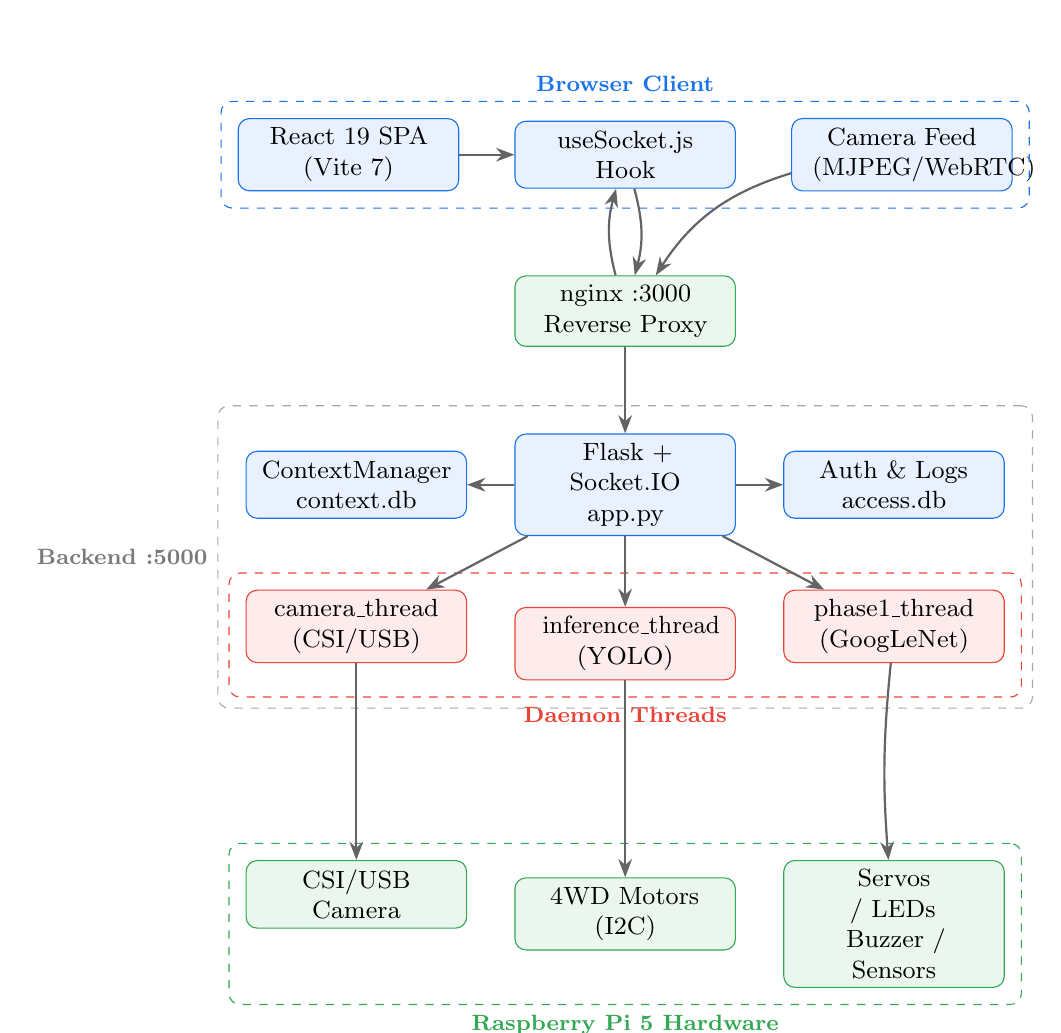
\begin{tikzpicture}[node distance=0.55cm and 0.7cm, font=\small]

  %% ── Browser layer ──
  \node[block, text width=2.2cm] (react) {React 19 SPA\\(Vite 7)};
  \node[block, right=of react, text width=2.2cm] (hook) {useSocket.js\\Hook};
  \node[block, right=of hook, text width=2.2cm] (cam_feed) {Camera Feed\\(MJPEG/WebRTC)};
  \node[draw=primary, dashed, rounded corners, fit=(react)(hook)(cam_feed),
        inner sep=6pt, label={[primary,font=\footnotesize\bfseries]above:Browser Client}] (browser) {};

  %% ── nginx ──
  \node[block2, below=1.1cm of hook, text width=2.2cm] (nginx)
        {nginx :3000\\Reverse Proxy};

  %% ── Backend ──
  \node[block, below=1.1cm of nginx, text width=2.4cm] (app)
        {Flask + Socket.IO\\app.py};
  \node[block, left=0.6cm of app, text width=2.4cm] (cm)
        {ContextManager\\context.db};
  \node[block, right=0.6cm of app, text width=2.4cm] (auth)
        {Auth \& Logs\\access.db};

  %% ── Thread pool ──
  \node[block3, below=0.9cm of cm, text width=2.1cm] (t1)
        {camera\_thread\\(CSI/USB)};
  \node[block3, below=0.9cm of app, text width=2.1cm] (t2)
        {inference\_thread\\(YOLO)};
  \node[block3, below=0.9cm of auth, text width=2.1cm] (t3)
        {phase1\_thread\\(GoogLeNet)};

  \node[draw=accent, dashed, rounded corners,
        fit=(t1)(t2)(t3), inner sep=6pt,
        label={[accent,font=\footnotesize\bfseries]below:Daemon Threads}] {};

  \node[draw=dark!40, dashed, rounded corners,
        fit=(app)(cm)(auth)(t1)(t2)(t3), inner sep=10pt,
        label={[dark!60,font=\footnotesize\bfseries]left:Backend :5000}] {};

  %% ── Hardware ──
  \node[block2, below=2.5cm of t1, text width=2.0cm] (hw_cam)
        {CSI/USB\\Camera};
  \node[block2, below=2.5cm of t2, text width=2.0cm] (hw_motor)
        {4WD Motors\\(I2C)};
  \node[block2, below=2.5cm of t3, text width=2.0cm] (hw_servo)
        {Servos / LEDs\\Buzzer / Sensors};
  \node[draw=secondary, dashed, rounded corners,
        fit=(hw_cam)(hw_motor)(hw_servo), inner sep=6pt,
        label={[secondary,font=\footnotesize\bfseries]below:Raspberry Pi 5 Hardware}] {};

  %% ── Arrows ──
  \draw[arrow] (react) -- (hook);
  \draw[arrow] (hook)  to[bend left=15] (nginx);
  \draw[arrow] (nginx) to[bend left=15] (hook);
  \draw[arrow] (cam_feed) to[bend right=20] (nginx);
  \draw[arrow] (nginx) -- (app);
  \draw[arrow] (app) -- (cm);
  \draw[arrow] (app) -- (auth);
  \draw[arrow] (app) -- (t1);
  \draw[arrow] (app) -- (t2);
  \draw[arrow] (app) -- (t3);
  \draw[arrow] (t1) -- (hw_cam);
  \draw[arrow] (t2) -- (hw_motor);
  \draw[arrow] (t3) to[bend right=5] (hw_servo);

\end{tikzpicture}
\caption{High-level system architecture. All real-time communication flows
through Socket.IO; the camera is streamed separately via MJPEG or WebRTC.}
\label{fig:arch_overview}
\end{figure}

\begin{tcolorbox}[colback=codebg, colframe=primary!40,
    title=Mermaid Source (system\_architecture.mmd), fonttitle=\footnotesize\bfseries,
    breakable]
\begin{lstlisting}[style=mermaid]
graph TB
  subgraph Browser["Browser Client"]
    UI["React 19 SPA (Vite 7)"]
    WS_CLIENT["Socket.IO Client"]
    MJPEG["MJPEG / WebRTC Camera Feed"]
  end
  subgraph Backend["Backend Flask :5000"]
    APP["app.py -- Flask + Socket.IO"]
    CM["ContextManager (context.db)"]
    Threads["camera | inference | phase1 | sensor | broadcast"]
  end
  subgraph Hardware["Raspberry Pi 5 Hardware"]
    CAM["CSI/USB Camera"]
    MOTOR["4WD Motors (I2C)"]
    ...
  end
  Browser <-->|"Socket.IO / WebSocket"| Backend
  Backend <-->|"Raspbot_Lib I2C / rpicam-vid"| Hardware
\end{lstlisting}
\end{tcolorbox}

\subsection{Threading Model}

The backend runs five concurrent daemon threads sharing state via Python
\texttt{threading.Lock} objects:

\begin{table}[H]
\centering
\caption{Backend daemon threads and their responsibilities.}
\label{tab:threads}
\begin{tabularx}{\linewidth}{@{}llX@{}}
\toprule
\textbf{Thread} & \textbf{Rate} & \textbf{Responsibility} \\
\midrule
\texttt{camera\_thread}    & 30 fps target & Reads YUV420 frames from \texttt{rpicam-vid} pipe (CSI) or OpenCV (USB); writes to shared \texttt{FrameManager} \\
\texttt{inference\_thread} & frame-driven  & Runs YOLO Phase~2 on new frames; deduplicates; emits \texttt{detection\_results} \\
\texttt{phase1\_thread}    & $\sim$1 Hz    & GoogLeNet Places365 scene recognition; triggers Phase~2 switch on stable scene \\
\texttt{sensor\_thread}    & $\sim$3 Hz    & Polls ultrasonic, IR, line-tracking via I2C; emits \texttt{sensors} \\
\texttt{broadcast\_thread} & $\sim$4 Hz    & Pushes robot status \& system metrics (CPU, RAM, temp) to all clients \\
\bottomrule
\end{tabularx}
\end{table}

%% ────────────────────────────────────────────────────────────
\section{Hardware Platform}
%% ────────────────────────────────────────────────────────────

\subsection{Yahboom Raspbot + Raspberry Pi 5}

\begin{table}[H]
\centering
\caption{Target hardware specifications.}
\label{tab:hardware}
\begin{tabular}{@{}ll@{}}
\toprule
\textbf{Component}     & \textbf{Specification} \\
\midrule
SBC                    & Raspberry Pi 5 (4 GB or 8 GB LPDDR4X) \\
CPU                    & ARM Cortex-A76 $\times$ 4, up to 2.4 GHz (aarch64) \\
OS                     & Raspberry Pi OS Bookworm (64-bit) \\
Camera                 & CSI module (\texttt{rpicam-vid}) or USB webcam (OpenCV) \\
Drive Control          & 4$\times$ DC motors, I2C motor driver (Raspbot\_Lib) \\
Servo                  & Pan (ID~1) + Tilt (ID~2), 0–180°, I2C \\
LED                    & WS2812 RGB strip (7 preset colours + custom RGB) \\
Buzzer                 & On/off + configurable pattern \\
Sensors                & Ultrasonic distance, 4-ch line-tracking, IR remote \\
Storage                & microSD (current) \\
\bottomrule
\end{tabular}
\end{table}

\begin{warnbox}[Storage Limitation — Action Required]
The Raspberry Pi~5 currently boots from a \textbf{microSD card} with limited
available capacity. The full \textbf{Objects365 frozen model set} (365 scene
models, each $\sim$25--50~MB per format variant) requires several gigabytes of
storage that exceeds the current card's free space. The Objects365 data has
been prepared and is available on \textbf{Google Drive} and \textbf{Google
Colab} for cloud-side benchmarking. \textbf{A high-capacity NVMe SSD (M.2
HAT+ or USB 3.0 enclosure) is planned for procurement} to enable full
on-device deployment of all model variants.
\end{warnbox}

%% ────────────────────────────────────────────────────────────
\section{Two-Phase Intelligence Pipeline}
%% ────────────────────────────────────────────────────────────

\subsection{Pipeline Overview}

\begin{figure}[H]
\centering
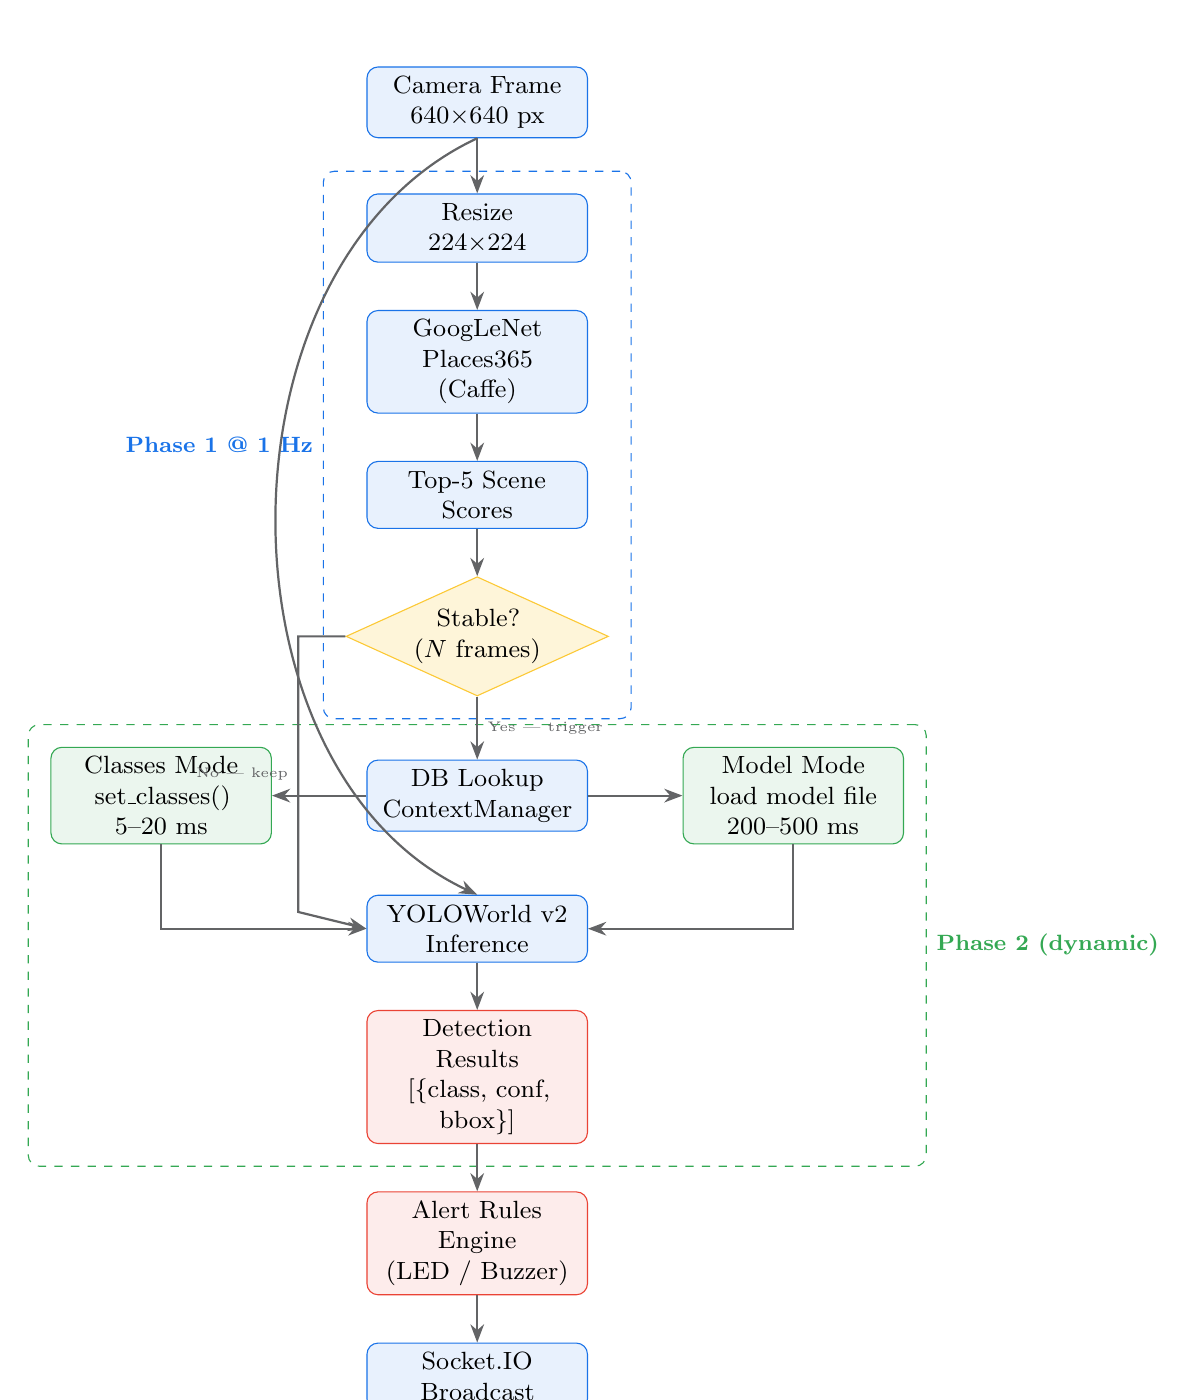
\begin{tikzpicture}[node distance=0.5cm and 0.8cm, font=\small]

  %% Input
  \node[block, text width=2.4cm] (cam) {Camera Frame\\640$\times$640 px};

  %% Phase 1
  \node[block, below=0.7cm of cam, text width=2.4cm] (resize)
        {Resize\\224$\times$224};
  \node[block, below=0.6cm of resize, text width=2.4cm] (goog)
        {GoogLeNet\\Places365 (Caffe)};
  \node[block, below=0.6cm of goog, text width=2.4cm] (top5)
        {Top-5 Scene Scores};
  \node[decision, below=0.6cm of top5, align=center, text width=1.6cm] (stable)
        {Stable? ($N$ frames)};
  \node[draw=primary, dashed, rounded corners,
        fit=(resize)(goog)(top5)(stable), inner sep=8pt,
        label={[primary,font=\footnotesize\bfseries]left:Phase 1 @ 1 Hz}] {};

  %% Phase 2
  \node[block, below=0.8cm of stable, text width=2.4cm] (db)
        {DB Lookup\\ContextManager};
  \node[block2, left=1.2cm of db, text width=2.2cm] (cls_mode)
        {Classes Mode\\set\_classes()\\5--20 ms};
  \node[block2, right=1.2cm of db, text width=2.2cm] (mdl_mode)
        {Model Mode\\load model file\\200--500 ms};
  \node[block, below=0.8cm of db, text width=2.4cm] (yolo)
        {YOLOWorld v2\\Inference};
  \node[block3, below=0.6cm of yolo, text width=2.4cm] (res)
        {Detection Results\\$[\{$class, conf, bbox$\}]$};
  \node[draw=secondary, dashed, rounded corners,
        fit=(db)(cls_mode)(mdl_mode)(yolo)(res), inner sep=8pt,
        label={[secondary,font=\footnotesize\bfseries]right:Phase 2 (dynamic)}] {};

  %% Alert
  \node[block3, below=0.6cm of res, text width=2.4cm] (alert)
        {Alert Rules Engine\\(LED / Buzzer)};

  %% Socket emit
  \node[block, below=0.6cm of alert, text width=2.4cm] (emit)
        {Socket.IO Broadcast};

  %% Arrows
  \draw[arrow] (cam) -- (resize);
  \draw[arrow] (resize) -- (goog);
  \draw[arrow] (goog) -- (top5);
  \draw[arrow] (top5) -- (stable);
  \draw[arrow] (stable) -- node[right, font=\tiny]{Yes — trigger} (db);
  \draw[arrow] (stable.west) -- +(-0.6,0) -- node[left,font=\tiny]{No — keep} +(-0.6,-3.5)
               -- (yolo.west);
  \draw[arrow] (db) -- (cls_mode);
  \draw[arrow] (db) -- (mdl_mode);
  \draw[arrow] (cls_mode) |- (yolo.west);
  \draw[arrow] (mdl_mode) |- (yolo.east);
  \draw[arrow] (cam.south) ++(0,0) to[bend right=65] (yolo.north);
  \draw[arrow] (yolo) -- (res);
  \draw[arrow] (res) -- (alert);
  \draw[arrow] (alert) -- (emit);

\end{tikzpicture}
\caption{Two-phase context-aware detection pipeline. Phase~1 runs at 1~Hz for
scene recognition; Phase~2 adapts YOLO classes based on the stable scene.}
\label{fig:pipeline}
\end{figure}

\begin{tcolorbox}[colback=codebg, colframe=secondary!40,
    title=Mermaid Source (phase1\_phase2\_pipeline.mmd), fonttitle=\footnotesize\bfseries,
    breakable]
\begin{lstlisting}[style=mermaid]
flowchart TD
    CAM["Camera Frame (640x640 px)"]
    subgraph P1["Phase 1 -- Scene Recognition (1 Hz)"]
        P1_DNN["GoogLeNet Places365 (Caffe)"]
        P1_STABLE{"Stable for N frames?"}
    end
    subgraph P2["Phase 2 -- Context-Aware Detection"]
        DB_LOOKUP["ContextManager.get_context_for_scene()"]
        M_CLASS["classes mode: set_classes() ~5-20 ms"]
        M_MODEL["model mode: Load model ~200-500 ms"]
        YOLO["YOLOWorld v2 Inference"]
    end
    CAM --> P1_DNN --> P1_STABLE
    P1_STABLE -->|"Yes"| DB_LOOKUP
    DB_LOOKUP --> M_CLASS & M_MODEL --> YOLO
    CAM --> YOLO --> RESULTS --> ALERT --> EMIT
\end{lstlisting}
\end{tcolorbox}

\subsection{Phase 1: Scene Recognition}

Phase~1 uses \textbf{GoogLeNet trained on Places365} (Caffe format, loaded via
OpenCV DNN) to classify the camera frame into one of \textbf{365 scene
categories}. Key parameters:

\begin{itemize}[leftmargin=*]
  \item Input resolution: $224 \times 224$ (resized from the $640 \times 640$
        capture frame)
  \item Output: Top-5 scene class scores with probability
  \item Target run rate: $\sim$1~Hz (triggered every $N$ inference frames)
  \item Stability threshold: 3 consecutive frames predicting the same scene
        before triggering Phase~2
  \item All predictions are logged to \texttt{phase1\_history} (SQLite) with
        UUID \texttt{infer\_id} and \texttt{inference\_ms}
\end{itemize}

\subsection{Phase 2: Context-Aware YOLO Detection}

When Phase~1 declares a stable scene, \texttt{\_switch\_scene()} is invoked:

\begin{enumerate}[leftmargin=*]
  \item Query \texttt{ContextManager.get\_context\_for\_scene(scene,
        vocabulary=\_context\_vocab)} — returns the YOLO class list and
        (optionally) an alternative model file.
  \item Switch the active YOLO model to the target classes via one of two modes:
\end{enumerate}

\begin{table}[H]
\centering
\caption{Phase~2 switch mode comparison.}
\label{tab:phase2_modes}
\begin{tabular}{@{}lll@{}}
\toprule
\textbf{Mode}   & \textbf{Mechanism}               & \textbf{Typical Latency} \\
\midrule
\texttt{classes} (default) & \texttt{yolo\_model.set\_classes(list)} & 5–20 ms \\
\texttt{model}             & Reload model file from disk            & 200–500 ms \\
\bottomrule
\end{tabular}
\end{table}

All switches are logged to \texttt{inference\_history} with a UUID
\texttt{switch\_id} and timing breakdown (\texttt{db\_query\_ms},
\texttt{switch\_ms}, \texttt{total\_ms}).

%% ────────────────────────────────────────────────────────────
\section{Dual-Vocabulary Context Architecture}
%% ────────────────────────────────────────────────────────────

\subsection{Motivation: The Vocabulary Ceiling Problem}

Standard YOLOv8 models operate on the COCO-80 vocabulary, which covers 80
common object categories. Many semantically important objects — \texttt{stethoscope},
\texttt{whiteboard}, \texttt{saxophone}, \texttt{cutting board} — have no COCO-80
equivalent, causing Phase~2 to silently ignore them.

The \textbf{Objects365} dataset (Shao et al., 2019) provides 365 fine-grained
categories that substantially expand coverage for specialised environments.

\subsection{Database Schema}

Both vocabularies are stored in a single \texttt{context.db} file for ACID
consistency and minimal Docker volume management:

\begin{figure}[H]
\centering
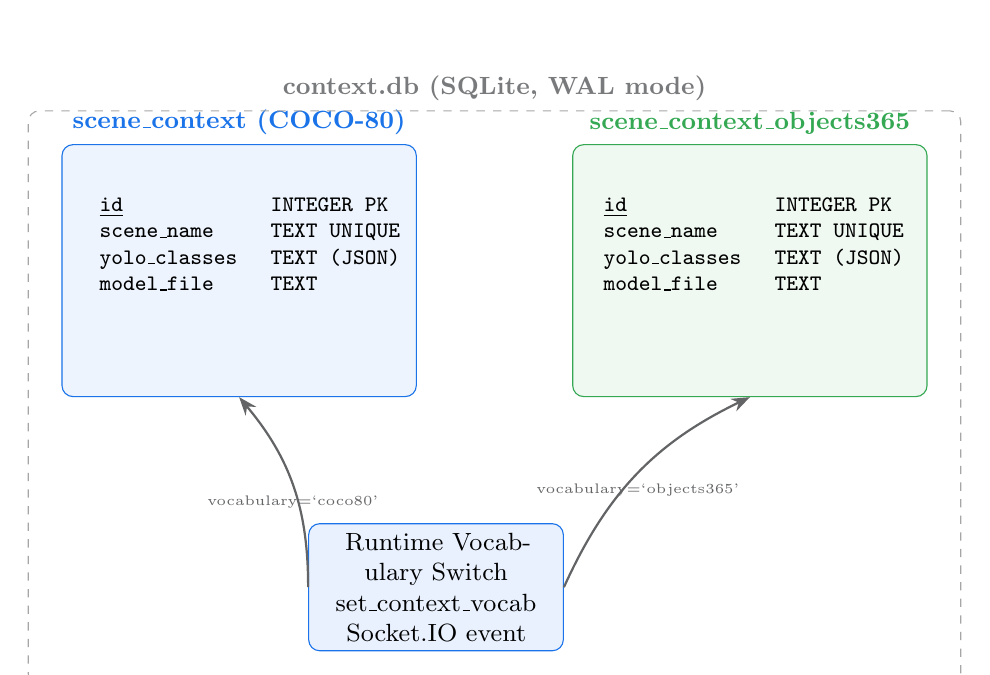
\begin{tikzpicture}[node distance=1.2cm and 2cm, font=\small]

  %% COCO table
  \node[draw=primary, rounded corners, fill=primary!8, minimum width=4.5cm,
        minimum height=3.2cm, label={[primary,font=\small\bfseries]above:scene\_context (COCO-80)},
        anchor=north west] (coco) at (0,0) {};
  \node[anchor=north west, font=\footnotesize\ttfamily] at (0.15,-0.5) {
    \begin{tabular}{ll}
      \underline{id}          & INTEGER PK \\
      scene\_name             & TEXT UNIQUE \\
      yolo\_classes           & TEXT (JSON) \\
      model\_file             & TEXT \\
    \end{tabular}
  };

  %% Objects365 table
  \node[draw=secondary, rounded corners, fill=secondary!8, minimum width=4.5cm,
        minimum height=3.2cm,
        label={[secondary,font=\small\bfseries]above:scene\_context\_objects365},
        anchor=north east] (o365) at (11,0) {};
  \node[anchor=north west, font=\footnotesize\ttfamily] at (6.55,-0.5) {
    \begin{tabular}{ll}
      \underline{id}          & INTEGER PK \\
      scene\_name             & TEXT UNIQUE \\
      yolo\_classes           & TEXT (JSON) \\
      model\_file             & TEXT \\
    \end{tabular}
  };

  %% vocab switch
  \node[block, below=1.6cm of coco.south, text width=3.0cm,
        xshift=2.5cm] (switch) {Runtime Vocabulary Switch\\set\_context\_vocab\\Socket.IO event};

  %% arrows
  \draw[arrow] (switch.west) to[bend right=20]
    node[below,font=\tiny]{vocabulary=`coco80'} (coco.south);
  \draw[arrow] (switch.east) to[bend left=20]
    node[below,font=\tiny]{vocabulary=`objects365'} (o365.south);

  %% context_db wrapper
  \node[draw=dark!40, dashed, rounded corners, fit=(coco)(o365)(switch),
        inner sep=12pt, label={[dark!60,font=\small\bfseries]above:context.db (SQLite, WAL mode)}] {};

\end{tikzpicture}
\caption{Dual-vocabulary database architecture. Both tables share an identical
schema; vocabulary selection is controlled at runtime via Socket.IO.}
\label{fig:dual_vocab}
\end{figure}

\begin{tcolorbox}[colback=codebg, colframe=dark!30,
    title=Mermaid Source (context\_manager.mmd), fonttitle=\footnotesize\bfseries]
\begin{lstlisting}[style=mermaid]
erDiagram
    SCENE_CONTEXT { text scene_name UK; text yolo_classes; text model_file }
    SCENE_CONTEXT_OBJECTS365 { text scene_name UK; text yolo_classes; text model_file }
    INFERENCE_HISTORY { text switch_id UK; text scene; text mode; real switch_ms }
    PHASE1_HISTORY { text infer_id UK; text scene; real confidence; real inference_ms }
    SCENE_CONTEXT ||--o{ INFERENCE_HISTORY : "scene lookup"
    PHASE1_HISTORY ||--o| INFERENCE_HISTORY : "triggers"
\end{lstlisting}
\end{tcolorbox}

\subsection{Vocabulary Coverage Analysis}

\begin{table}[H]
\centering
\caption{Class coverage comparison: COCO-80 vs.\ Objects365 per scene.}
\label{tab:vocab_coverage}
\begin{tabularx}{\linewidth}{@{}lccX@{}}
\toprule
\textbf{Scene}     & \textbf{COCO-80} & \textbf{Objects365} & \textbf{Examples unique to Objects365} \\
\midrule
living\_room  & 14 & 32 & carpet, lamp, pillow, blanket, curtain, magazine \\
kitchen       & 13 & 22 & faucet, kettle, blender, gas stove, cutting board \\
office        & 10 & 22 & monitor, tablet, printer, whiteboard, ruler, stapler \\
hospital      &  6 & 16 & wheelchair, stethoscope, syringe, thermometer, bandage \\
street        & 12 & 19 & SUV, street lights, traffic cone, mailbox \\
concert       &  0 & 11 & guitar, violin, piano, drum, saxophone, microphone \\
\midrule
\textbf{Average} & \textbf{9.2} & \textbf{17.5} & \textbf{$\approx$1.9$\times$ more classes/scene} \\
\bottomrule
\end{tabularx}
\end{table}

\begin{figure}[H]
\centering
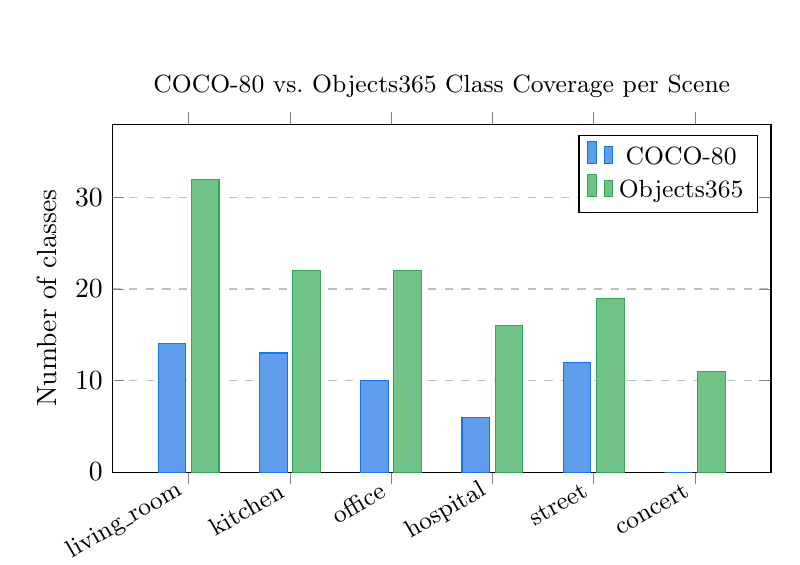
\begin{tikzpicture}
\begin{axis}[
  ybar,
  width=0.82\linewidth, height=6cm,
  bar width=10pt,
  symbolic x coords={living\_room, kitchen, office, hospital, street, concert},
  xtick=data,
  x tick label style={rotate=30, anchor=east, font=\small},
  legend style={at={(0.98,0.97)}, anchor=north east, font=\small},
  ylabel={Number of classes},
  ymin=0, ymax=38,
  ymajorgrids=true,
  grid style=dashed,
  enlarge x limits=0.15,
  title={\small COCO-80 vs.\ Objects365 Class Coverage per Scene}
]
\addplot[fill=primary!70, draw=primary] coordinates {
  (living\_room,14) (kitchen,13) (office,10)
  (hospital,6) (street,12) (concert,0)
};
\addplot[fill=secondary!70, draw=secondary] coordinates {
  (living\_room,32) (kitchen,22) (office,22)
  (hospital,16) (street,19) (concert,11)
};
\legend{COCO-80, Objects365}
\end{axis}
\end{tikzpicture}
\caption{Objects365 provides on average 1.9$\times$ more detectable classes per
scene, with especially large gains for medical, musical, and indoor scenes.}
\label{fig:vocab_bar}
\end{figure}

%% ────────────────────────────────────────────────────────────
\section{YOLO Model Benchmark}
%% ────────────────────────────────────────────────────────────

\subsection{Model Formats Evaluated}

All models are derived from \textbf{YOLOv8n (nano)} and evaluated on the
Raspberry Pi~5 CPU (ARM Cortex-A76) with input size $640 \times 640$, test
image: \texttt{bus.jpg} (4 persons, 1 bus).

\begin{table}[H]
\centering
\caption{Inference benchmark results on Raspberry Pi~5 CPU.}
\label{tab:benchmark}
\begin{tabular}{@{}llccc@{}}
\toprule
\textbf{Model File}    & \textbf{Format}      & \textbf{Inference (ms)} & \textbf{Detections} & \textbf{Notes} \\
\midrule
yolo26n\_float16.tflite & TFLite float16      & \textbf{302.0}          & 4p + 1b & XNNPACK delegate \\
yolo26n\_float32.tflite & TFLite float32      & 309.1                   & 4p + 1b & XNNPACK delegate \\
yolo26n.onnx            & ONNX Runtime 1.24.1 & 420.3                   & 4p + 1b & CPUExecutionProvider \\
yolo26n.pt              & PyTorch (ultralytics)& 460.8                  & 4p + 1b & torch 2.10.0+cpu \\
\bottomrule
\end{tabular}
\end{table}

\begin{figure}[H]
\centering
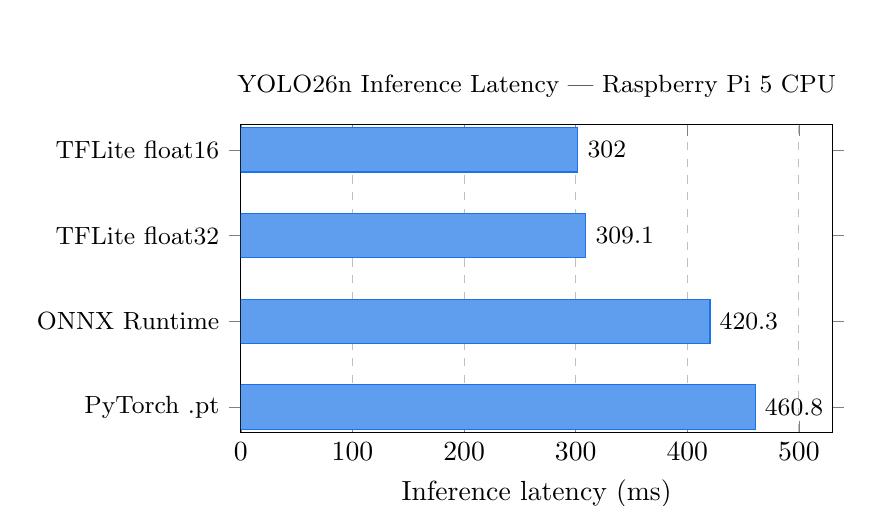
\begin{tikzpicture}
\begin{axis}[
  xbar,
  width=0.75\linewidth, height=5.5cm,
  bar width=16pt,
  ytick={1,2,3,4},
  yticklabels={PyTorch .pt, ONNX Runtime, TFLite float32, TFLite float16},
  y tick label style={font=\small},
  xlabel={Inference latency (ms)},
  xmin=0, xmax=530,
  xmajorgrids=true,
  grid style=dashed,
  nodes near coords,
  nodes near coords align={horizontal},
  every node near coord/.style={font=\small},
  title={\small YOLO26n Inference Latency --- Raspberry Pi 5 CPU}
]
\addplot[fill=primary!70, draw=primary] coordinates {
  (460.8, 1)
  (420.3, 2)
  (309.1, 3)
  (302.0, 4)
};
\end{axis}
\end{tikzpicture}
\caption{TFLite float16 achieves the fastest inference at 302 ms, a
35\% improvement over PyTorch. XNNPACK delegate enables ARM-optimised SIMD
execution for TFLite on Cortex-A76.}
\label{fig:benchmark_bar}
\end{figure}

\begin{resultbox}[Key Finding]
\textbf{TFLite float16} is the recommended deployment format for Raspberry Pi 5.
It achieves the lowest latency (302~ms) while maintaining identical detection
output (4 persons + 1 bus). The ONNX Runtime is a viable alternative at
420~ms without requiring TensorFlow Lite. The full Objects365 model benchmark
(365+ model variants) is available on \textbf{Google Drive} and
\textbf{Google Colab} — see Section~\ref{sec:results_location}.
\end{resultbox}

%% ────────────────────────────────────────────────────────────
\section{Communication Architecture}
%% ────────────────────────────────────────────────────────────

\subsection{Socket.IO Event Map}

\begin{table}[H]
\centering
\caption{Key Socket.IO events (C = client$\to$server; S = server$\to$client).}
\label{tab:socketio}
\small
\begin{tabularx}{\linewidth}{@{}llX@{}}
\toprule
\textbf{Event}         & \textbf{Dir.} & \textbf{Payload / Purpose} \\
\midrule
\texttt{authenticate}  & C & \texttt{\{password\}} — unlock control commands \\
\texttt{move}          & C & \texttt{\{direction: forward|backward|left|right|...\}} \\
\texttt{stop}          & C & Emergency stop \\
\texttt{servo}         & C & \texttt{\{id: 1|2, angle: 0--180\}} \\
\texttt{speed}         & C & \texttt{\{speed: 0--255\}} \\
\texttt{led}           & C & \texttt{\{action, color: 0--6\}} \\
\texttt{detection\_toggle}   & C & \texttt{\{enabled: bool\}} \\
\texttt{set\_scene}    & C & \texttt{\{scene: 'kitchen'\}} — manual Phase~2 override \\
\texttt{set\_context\_vocab} & C & \texttt{\{vocab: 'coco80'|'objects365'\}} \\
\texttt{alert\_rules\_sync}  & C & Full-replace alert rules array \\
\midrule
\texttt{status}        & S & Robot state broadcast @ 4~Hz \\
\texttt{sensors}       & S & Ultrasonic, IR, line-tracking @ 3~Hz \\
\texttt{detection\_results} & S & YOLO results per inference frame \\
\texttt{phase1\_result}     & S & Top-5 Places365 scene predictions \\
\texttt{phase2\_timing}     & S & \texttt{\{switch\_id, scene, mode, db\_ms, switch\_ms\}} \\
\texttt{alert\_triggered}   & S & Alert rule fired \\
\bottomrule
\end{tabularx}
\end{table}

\subsection{Camera Streaming: MJPEG vs.\ WebRTC}

\begin{table}[H]
\centering
\caption{Camera transport mechanism comparison.}
\label{tab:streaming}
\begin{tabular}{@{}llll@{}}
\toprule
\textbf{Property}          & \textbf{MJPEG (current)} & \textbf{WebRTC (experimental)} \\
\midrule
Transport                  & TCP (HTTP chunked)       & UDP (DTLS/SRTP RTP) \\
Codec                      & JPEG per frame           & H.264 / VP8 / VP9 \\
Compression                & Spatial only (DCT)       & Spatial + temporal \\
Typical bitrate            & 2--5 Mbps                & 200--600 kbps \\
Glass-to-glass latency     & 500 ms -- 2 s            & $<$200 ms \\
Head-of-line blocking      & Yes (TCP)                & No (UDP discard) \\
Browser decode             & Software                 & GPU-accelerated \\
Implementation complexity  & Low                      & High (aiortc, asyncio) \\
Status                     & \textbf{Production}      & Experimental \\
\bottomrule
\end{tabular}
\end{table}

The end-to-end latency models for the two transports are:
\begin{align}
L_{\text{MJPEG}}  &= t_{\text{cap}} + t_{\text{JPEG}} + t_{\text{TCP buffer}} + t_{\text{render}} \\
L_{\text{WebRTC}} &= t_{\text{cap}} + t_{\text{encode}} + t_{\text{UDP}} + t_{\text{decode}}
\end{align}

%% ────────────────────────────────────────────────────────────
\section{Frontend Architecture}
%% ────────────────────────────────────────────────────────────

\subsection{Component Overview}

\begin{figure}[H]
\centering
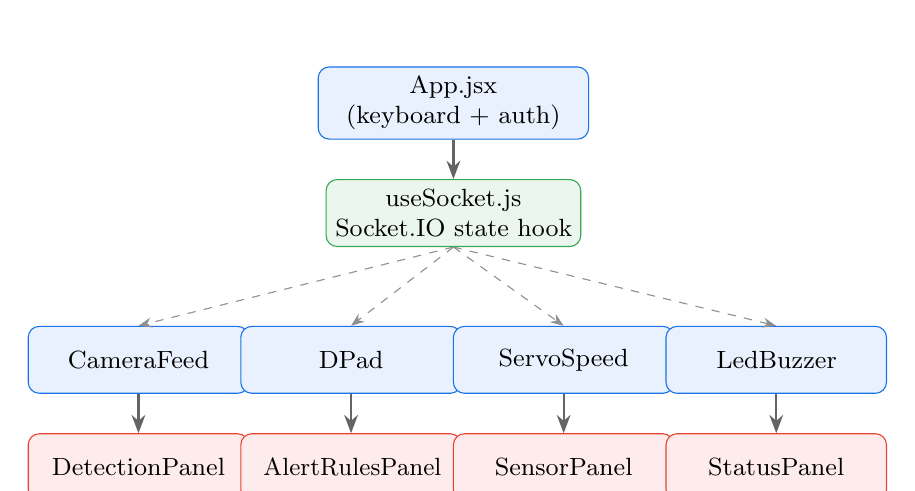
\begin{tikzpicture}[node distance=0.45cm and 0.5cm, font=\small]

  \node[block, text width=3.2cm, minimum height=0.9cm] (app)
        {App.jsx\\(keyboard + auth)};

  \node[block2, below=0.5cm of app, text width=3.0cm] (hook)
        {useSocket.js\\Socket.IO state hook};

  %% Component row 1
  \node[block, below=1.0cm of hook, text width=2.2cm, xshift=-4cm] (cam)
        {CameraFeed};
  \node[block, below=1.0cm of hook, text width=2.2cm, xshift=-1.3cm] (dpad)
        {DPad};
  \node[block, below=1.0cm of hook, text width=2.2cm, xshift=1.4cm] (servo)
        {ServoSpeed};
  \node[block, below=1.0cm of hook, text width=2.2cm, xshift=4.1cm] (led)
        {LedBuzzer};

  %% Component row 2
  \node[block3, below=0.5cm of cam, text width=2.2cm] (det)
        {DetectionPanel};
  \node[block3, below=0.5cm of dpad, text width=2.2cm] (alert)
        {AlertRulesPanel};
  \node[block3, below=0.5cm of servo, text width=2.2cm] (sens)
        {SensorPanel};
  \node[block3, below=0.5cm of led, text width=2.2cm] (stat)
        {StatusPanel};

  %% Arrows
  \draw[arrow] (app) -- (hook);
  \draw[dasharrow] (hook.south) -- (cam.north);
  \draw[dasharrow] (hook.south) -- (dpad.north);
  \draw[dasharrow] (hook.south) -- (servo.north);
  \draw[dasharrow] (hook.south) -- (led.north);
  \draw[arrow] (cam) -- (det);
  \draw[arrow] (dpad) -- (alert);
  \draw[arrow] (servo) -- (sens);
  \draw[arrow] (led) -- (stat);

\end{tikzpicture}
\caption{Frontend React component tree. \texttt{useSocket.js} distributes
Socket.IO state; \texttt{App.jsx} coordinates keyboard/auth logic.}
\label{fig:frontend}
\end{figure}

\begin{tcolorbox}[colback=codebg, colframe=dark!30,
    title=Mermaid Source (frontend\_dataflow.mmd), fonttitle=\footnotesize\bfseries,
    breakable]
\begin{lstlisting}[style=mermaid]
sequenceDiagram
    participant User
    participant App as App.jsx (React)
    participant Hook as useSocket.js
    participant IO as Socket.IO Server
    participant HW as Hardware (Raspbot_Lib)

    User->>App: Press WASD / touch D-pad
    App->>Hook: emit('move', {direction})
    Hook->>IO: WebSocket frame
    IO->>HW: Car.set_motor() via I2C
    IO-->>Hook: broadcast 'status' @ 4 Hz
    Hook-->>App: setStatus(newState)
    App-->>User: UI reflects motor state
\end{lstlisting}
\end{tcolorbox}

%% ────────────────────────────────────────────────────────────
\section{Alert Rules Engine}
%% ────────────────────────────────────────────────────────────

The alert system allows the robot to autonomously respond when specific objects
are detected above a configurable threshold.

\begin{table}[H]
\centering
\caption{Alert rule structure.}
\label{tab:alert}
\begin{tabular}{@{}lll@{}}
\toprule
\textbf{Field}       & \textbf{Type}   & \textbf{Description} \\
\midrule
\texttt{id}           & UUID string  & Unique rule identifier \\
\texttt{class\_name}  & string       & YOLO class to watch (e.g., \texttt{person}) \\
\texttt{count\_threshold} & int      & Trigger when count $\ge$ threshold \\
\texttt{action\_type} & string       & \texttt{led\_color}, \texttt{led\_rgb}, \texttt{buzzer\_on}, \texttt{buzzer\_pattern} \\
\texttt{action\_params} & dict       & e.g., \texttt{\{on\_ms: 200, off\_ms: 200, repeats: 3\}} \\
\texttt{enabled}      & bool         & Rule active flag \\
\bottomrule
\end{tabular}
\end{table}

Rising-edge detection triggers the action after $N$ consecutive frames meeting
the threshold; falling-edge clears it after $N$ frames below threshold.
Anti-flicker via \texttt{alert\_cooldown} counter prevents rapid on/off
oscillation.

%% ────────────────────────────────────────────────────────────
\section{Docker Deployment Architecture}
%% ────────────────────────────────────────────────────────────

\begin{figure}[H]
\centering
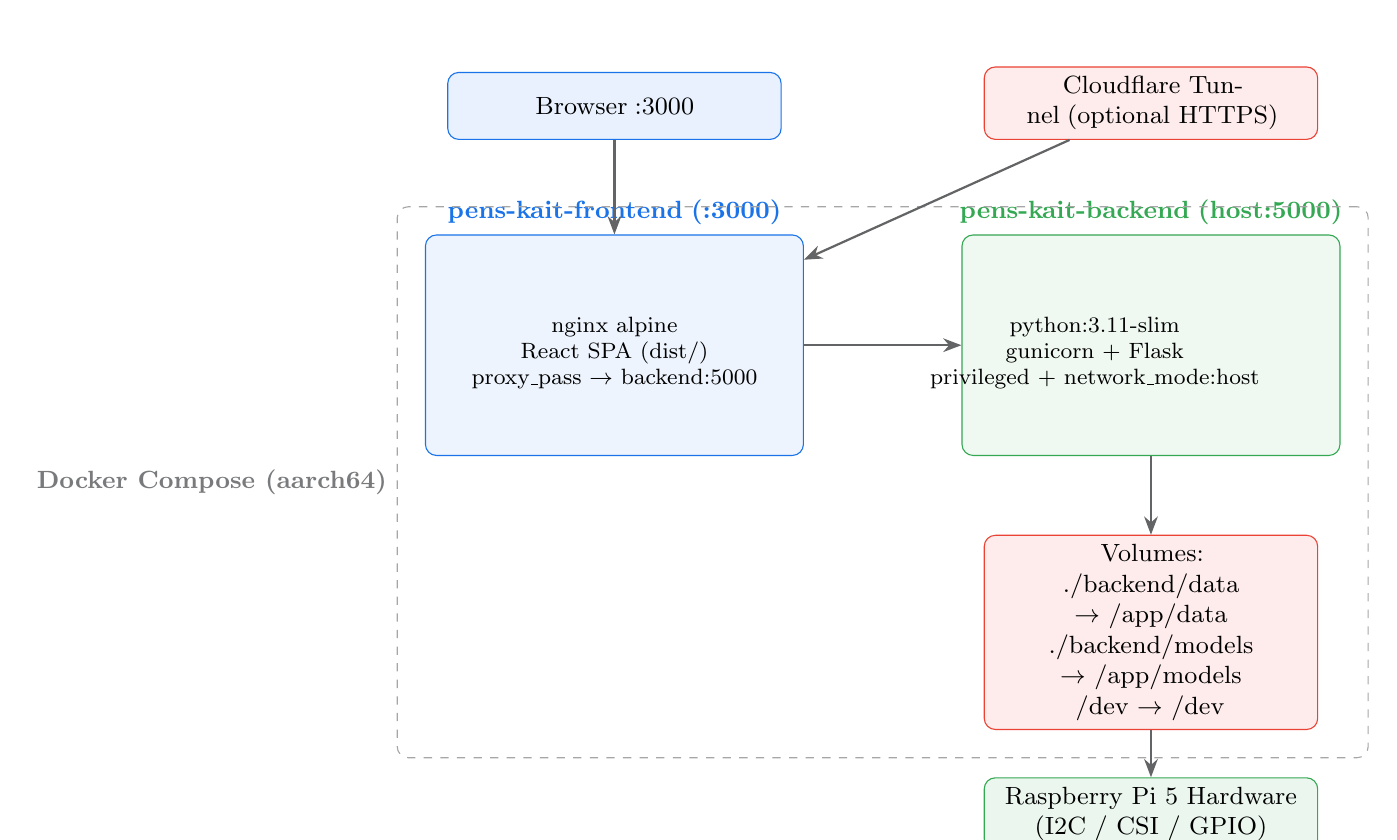
\begin{tikzpicture}[node distance=0.6cm and 0.8cm, font=\small]

  %% Frontend container
  \node[draw=primary, rounded corners, fill=primary!8, minimum width=4.8cm,
        minimum height=2.8cm,
        label={[primary,font=\small\bfseries]above:pens-kait-frontend\;(:3000)}]
        (fe) at (0,0) {};
  \node[font=\footnotesize, anchor=center] at (0,-0.1) {
    \begin{tabular}{c}
      nginx alpine \\
      React SPA (dist/) \\
      proxy\_pass $\to$ backend:5000
    \end{tabular}
  };

  %% Backend container
  \node[draw=secondary, rounded corners, fill=secondary!8, minimum width=4.8cm,
        minimum height=2.8cm,
        label={[secondary,font=\small\bfseries]above:pens-kait-backend\;(host:5000)},
        right=2cm of fe] (be) {};
  \node[font=\footnotesize, anchor=center] at (6.1,-0.1) {
    \begin{tabular}{c}
      python:3.11-slim \\
      gunicorn + Flask \\
      privileged + network\_mode:host
    \end{tabular}
  };

  %% Volumes
  \node[block3, below=1.0cm of be.south, text width=4.0cm, xshift=0] (vol)
        {Volumes:\\./backend/data $\to$ /app/data\\./backend/models $\to$ /app/models\\ /dev $\to$ /dev};

  %% Hardware
  \node[block2, below=0.6cm of vol, text width=4.0cm] (hw)
        {Raspberry Pi 5 Hardware\\(I2C / CSI / GPIO)};

  %% Browser
  \node[block, above=1.2cm of fe, text width=4.0cm] (browser)
        {Browser\;:3000};

  %% Cloudflare
  \node[block3, above=1.2cm of be, text width=4.0cm] (cf)
        {Cloudflare Tunnel\;(optional HTTPS)};

  %% Docker Compose boundary
  \node[draw=dark!40, dashed, rounded corners,
        fit=(fe)(be)(vol), inner sep=10pt,
        label={[dark!60,font=\small\bfseries]left:Docker Compose (aarch64)}] {};

  %% Arrows
  \draw[arrow] (browser) -- (fe);
  \draw[arrow] (fe.east) -- (be.west);
  \draw[arrow] (be.south) -- (vol.north);
  \draw[arrow] (vol.south) -- (hw.north);
  \draw[arrow] (cf) -- (fe);

\end{tikzpicture}
\caption{Docker Compose deployment. Backend uses \texttt{network\_mode: host}
and \texttt{privileged: true} for hardware access. Volumes persist SQLite
databases and model files across container restarts.}
\label{fig:docker}
\end{figure}

\begin{tcolorbox}[colback=codebg, colframe=dark!30,
    title=Mermaid Source (docker\_deployment.mmd), fonttitle=\footnotesize\bfseries]
\begin{lstlisting}[style=mermaid]
graph TB
  subgraph DC["Docker Compose (aarch64)"]
    FE["pens-kait-frontend :3000\nnginx + React SPA\nproxy_pass -> backend:5000"]
    BE["pens-kait-backend :5000\ngunicorn + Flask\nprivileged: true, network_mode: host"]
  end
  FE <-->|proxy_pass| BE
  BE <-->|"smbus2 I2C / rpicam-vid"| HW["Raspberry Pi 5 Hardware"]
  BROWSER -->|"HTTP :3000"| FE
  CF["Cloudflare Tunnel (optional)"] --> FE
\end{lstlisting}
\end{tcolorbox}

\subsection{Build \& Run Commands}

\begin{tcolorbox}[colback=dark!95, colframe=dark,
    title=Docker Compose Commands, fonttitle=\small\bfseries\color{white},
    colupper=white]
\begin{lstlisting}[style=shell]
# Build and start both containers
sudo docker compose up --build

# Run detached (production)
sudo docker compose up -d

# Access dashboard: http://<pi-ip>:3000

# Backend local dev
cd backend && python -m venv .venv && source .venv/bin/activate
pip install -r requirements.txt && cp .env.example .env
python app.py   # http://localhost:5000

# Frontend local dev
cd frontend && npm install && npm run dev  # http://localhost:5173
\end{lstlisting}
\end{tcolorbox}

%% ────────────────────────────────────────────────────────────
\section{Storage Limitation \& Procurement Plan}
\label{sec:storage}
%% ────────────────────────────────────────────────────────────

\begin{warnbox}[Current Storage Constraint]
The system currently runs on a \textbf{microSD card} with limited available
capacity. The following storage demands exceed what is currently available
on-device:

\begin{itemize}[leftmargin=*]
  \item \textbf{Objects365 frozen model set}: 365 scene-specific YOLO model
        variants, each exported in multiple formats (PyTorch, ONNX, TFLite
        float32, TFLite float16). Estimated total: \textbf{15--50 GB}.
  \item \textbf{YOLO training outputs} (\texttt{runs/}): Checkpoints,
        tensorboard logs, and prediction outputs from model fine-tuning.
  \item \textbf{NCNN and OpenVINO format caches}: Compiled models for
        additional inference backends.
\end{itemize}
\end{warnbox}

\subsection{Interim Solution: Google Drive \& Google Colab}
\label{sec:results_location}

While hardware procurement is pending, all model training, format conversion,
and benchmarking for the full Objects365 model set is performed in
\textbf{Google Colab} (A100/T4 GPU environment) and stored on
\textbf{Google Drive}. This includes:

\begin{itemize}[leftmargin=*]
  \item Full benchmark results table (all 365 scene models $\times$ 4 formats)
  \item Training logs and validation curves
  \item Exported model files (.pt, .onnx, .tflite float32/float16)
  \item Performance comparison notebooks
\end{itemize}

\begin{infobox}[Access to Results]
  \textbf{Google Drive:} Full model set, benchmark CSVs, and exported models\\
  \textbf{Google Colab:} Benchmark notebooks, training scripts, format
  conversion pipeline
  \\[0.4em]
  \textit{Links will be shared in the seminar session.}
\end{infobox}

\subsection{Procurement Plan}

\begin{table}[H]
\centering
\caption{Recommended storage upgrade options for Raspberry Pi 5.}
\label{tab:storage}
\begin{tabular}{@{}llll@{}}
\toprule
\textbf{Option}            & \textbf{Interface}  & \textbf{Capacity}  & \textbf{Notes} \\
\midrule
M.2 NVMe (M.2 HAT+)       & PCIe 2.0 $\times$1  & 256 GB -- 2 TB     & Best performance, $\sim$400 MB/s \\
USB 3.0 SSD (external)    & USB 3.0             & 480 GB -- 2 TB     & Portable, no HAT required \\
High-speed microSD (A2)   & UHS-I / SDR104      & 128--512 GB        & Minimal modification \\
\bottomrule
\end{tabular}
\end{table}

The \textbf{M.2 NVMe via M.2 HAT+} is strongly recommended: it mounts directly
to the Raspberry Pi~5 PCIe connector, offers sequential read speeds of
$\sim$400~MB/s (vs. $\sim$90~MB/s on microSD), and provides ample capacity
for all model variants and training runs.

%% ────────────────────────────────────────────────────────────
\section{Performance Summary}
%% ────────────────────────────────────────────────────────────

\begin{table}[H]
\centering
\caption{Key performance metrics vs.\ targets.}
\label{tab:perf}
\begin{tabular}{@{}llll@{}}
\toprule
\textbf{Metric}                          & \textbf{Target}   & \textbf{Measured}        & \textbf{Status} \\
\midrule
Control latency (keypress $\to$ motor)   & $<$100 ms         & $\sim$50--80 ms (LAN)    & \textcolor{secondary}{\checkmark} \\
Camera capture FPS                       & 30 fps            & 24--30 fps               & \textcolor{secondary}{\checkmark} \\
YOLO inference (yolo26n, TFLite f16)    & fastest achievable & 302 ms                   & \textcolor{secondary}{\checkmark} \\
YOLO inference (yolo26n, ONNX)          & —                 & 420 ms                   & — \\
YOLO inference (yolo26n, PyTorch)       & —                 & 461 ms                   & — \\
Phase~1 GoogLeNet inference             & $\sim$1 Hz rate   & 50--100 ms               & \textcolor{secondary}{\checkmark} \\
Phase~2 switch (classes mode)           & $<$3 s            & 5--20 ms                 & \textcolor{secondary}{\checkmark} \\
Phase~2 switch (model mode)             & $<$3 s            & 200--500 ms              & \textcolor{secondary}{\checkmark} \\
Backend memory footprint                & $<$1.5 GB         & $\sim$0.8--1.2 GB        & \textcolor{secondary}{\checkmark} \\
\bottomrule
\end{tabular}
\end{table}

%% ────────────────────────────────────────────────────────────
\section{Current Limitations \& Future Work}
%% ────────────────────────────────────────────────────────────

\begin{enumerate}[leftmargin=*, label=\textbf{L\arabic*.}]

  \item \textbf{CPU-only inference}: YOLO runs on the ARM Cortex-A76 without
        hardware acceleration. Exploratory Vulkan compute work
        (\texttt{backend/vulkan\_test.py}) targeting the VideoCore~VII GPU
        is in progress. A successful implementation could reduce inference
        latency from 302~ms to $<$50~ms.

  \item \textbf{Storage constraint}: As described in Section~\ref{sec:storage},
        NVMe SSD procurement is required to deploy the full Objects365 model
        set on-device.

  \item \textbf{WebRTC in production}: The aiortc integration is experimental;
        ICE candidate handling and TURN server configuration need finalisation
        for non-LAN deployments.

  \item \textbf{NCNN format}: NCNN-format models
        (\texttt{yolo26n\_ncnn\_model/}) are generated but not yet integrated
        into the inference pipeline — a promising path for further latency
        reduction.

  \item \textbf{YOLOWorld fine-tuning}: The current Objects365 vocabulary
        mapping uses pre-trained class embeddings. Fine-tuning
        YOLOWorld on domain-specific data (e.g., medical or industrial scenes)
        is planned.

\end{enumerate}

%% ────────────────────────────────────────────────────────────
\section{Conclusion}
%% ────────────────────────────────────────────────────────────

PENS-KAIT 2026 demonstrates a complete, deployable \textbf{context-aware robot
control platform} on Raspberry Pi~5. The core contributions presented in this
seminar report are:

\begin{itemize}[leftmargin=*]
  \item A working \textbf{two-phase detection pipeline} combining Places365
        scene recognition with dynamic YOLOWorld class switching.
  \item A \textbf{dual-vocabulary context database} (COCO-80 + Objects365)
        providing 1.9$\times$ greater class coverage per scene.
  \item A \textbf{benchmark} showing TFLite float16 achieves 302~ms inference
        — 35\% faster than PyTorch — on Raspberry Pi~5 CPU.
  \item A \textbf{production-ready Docker deployment} with authenticated
        Socket.IO control, MJPEG streaming, alert rules, and a full React
        dashboard.
  \item An \textbf{experimental WebRTC subsystem} reducing streaming latency
        from 500~ms--2~s (MJPEG) to $<$200~ms.
\end{itemize}

The immediate next steps are NVMe SSD procurement to enable full on-device
model deployment and Vulkan GPU compute integration for sub-50~ms YOLO
inference.

%% ────────────────────────────────────────────────────────────
\appendix
\section{File Structure Reference}
%% ────────────────────────────────────────────────────────────

\begin{small}
\begin{verbatim}
PENS-KAIT 2026/
+-- backend/
|   +-- app.py                   # Main server (Flask + Socket.IO, 1975 lines)
|   +-- context_manager.py       # Scene-to-class DB manager (621 lines)
|   +-- requirements.txt
|   +-- Dockerfile
|   +-- data/
|   |   +-- context.db           # SQLite: scene_context + scene_context_objects365
|   |   +-- access.db            # SQLite: access_log + inference_history + phase1_history
|   |   \-- places365.csv        # Places365 scene category CSV (seed data)
|   \-- models/
|       +-- phase1_model.py      # GoogLeNet Places365 inference wrapper
|       +-- yolo26n.pt/.onnx     # YOLOv8 nano (PyTorch / ONNX)
|       +-- yolo26n_saved_model/ # TFLite float32 + float16
|       +-- yolov8s-worldv2.pt   # YOLOWorld (dynamic class setting)
|       \-- Phase1/              # GoogLeNet Caffe weights + prototxt
+-- frontend/
|   +-- src/
|   |   +-- App.jsx              # Main app (keyboard, auth)
|   |   +-- hooks/useSocket.js   # Socket.IO state management
|   |   \-- components/          # CameraFeed, DPad, ServoSpeed, DetectionPanel, ...
|   \-- Dockerfile               # Multi-stage: node:20 -> nginx:alpine
+-- docker-compose.yaml
+-- docs/
|   +-- seminar/                 # This document
|   |   +-- main.tex
|   |   +-- build.sh
|   |   \-- diagrams/*.mmd       # Mermaid source files
|   \-- system_progress_report_*.md/.pdf
\-- PRD.md                       # Product Requirements Document
\end{verbatim}
\end{small}

%% ────────────────────────────────────────────────────────────
\section{Environment Variables}
%% ────────────────────────────────────────────────────────────

\begin{table}[H]
\centering
\caption{\texttt{backend/.env} configuration variables.}
\begin{tabular}{@{}lll@{}}
\toprule
\textbf{Variable}          & \textbf{Default}    & \textbf{Description} \\
\midrule
\texttt{ADMIN\_PASSWORD}   & (required)          & Dashboard unlock password \\
\texttt{CAMERA\_TYPE}      & \texttt{AUTO}       & \texttt{CSI} | \texttt{USB} | \texttt{AUTO} \\
\texttt{TURNSTILE\_SECRET\_KEY} & (optional)     & Cloudflare Turnstile secret \\
\texttt{TURNSTILE\_SITE\_KEY}   & (optional)     & Cloudflare Turnstile public key \\
\bottomrule
\end{tabular}
\end{table}

\end{document}
